\documentclass[10pt,a4paper,landscape]{article}
\usepackage[margin=15mm,headheight=14pt,headsep=5mm,footskip=8mm]{geometry}
\usepackage[T1]{fontenc}
\usepackage{lmodern,microtype,xcolor,tikz,tabularx,booktabs,array,fancyhdr,hyperref,amsmath}
\usetikzlibrary{arrows.meta,positioning}
\renewcommand{\familydefault}{\sfdefault}
\definecolor{navy}{HTML}{183447}
\definecolor{teal}{HTML}{147B80}
\definecolor{pale}{HTML}{EDF6F5}
\definecolor{slate}{HTML}{526574}
\definecolor{rulegray}{HTML}{CDDDE2}
\definecolor{sand}{HTML}{FCF3E4}
\definecolor{plotblue}{HTML}{176B94}
\definecolor{plotorange}{HTML}{BD601C}
\hypersetup{colorlinks=true,urlcolor=teal,pdftitle={FININ-inspired news prediction: current progress},pdfauthor={Research progress report}}
\pagestyle{fancy}\fancyhf{}
\fancyhead[L]{\small\color{slate}FININ-INSPIRED NEWS PREDICTION / MEETING REPORT}
\fancyhead[R]{\small\color{slate}14 OCTOBER 2026}
\fancyfoot[L]{\scriptsize\color{slate}Public CMIN-US adaptation / exploratory chronological evaluation}
\fancyfoot[R]{\small\color{slate}\thepage\ / 3}
\renewcommand{\headrulewidth}{0pt}
\setlength{\parindent}{0pt}\setlength{\parskip}{4pt}
\renewcommand{\arraystretch}{1.08}\setlength{\tabcolsep}{7pt}
\newcolumntype{Y}{>{\raggedright\arraybackslash}X}
\newcolumntype{P}[1]{>{\raggedright\arraybackslash}p{#1}}
\newcommand{\heading}[1]{{\fontsize{23}{27}\selectfont\bfseries\color{navy}#1}\par}
\newcommand{\sub}[1]{\vspace{3pt}{\large\bfseries\color{navy}#1}\par}
\newcommand{\callout}[1]{\par\colorbox{pale}{\parbox{\dimexpr\linewidth-2\fboxsep}{\vspace{4pt}#1\vspace{4pt}}}\par}
\newcommand{\caution}[1]{\par\colorbox{sand}{\parbox{\dimexpr\linewidth-2\fboxsep}{\vspace{4pt}#1\vspace{4pt}}}\par}
\newcommand{\NoInteractionLoss}{0.693387}
\newcommand{\InteractionDelta}{+0.002999}
\newcommand{\InteractionInterval}{[+0.001058, +0.005092]}
\newcommand{\InteractionVerdict}{The pooled comparison favors interactions, but period means disagree and the average effect is below the 0.005 practical criterion. Full still trails prices (0.690095).}
\tikzset{box/.style={draw=rulegray,rounded corners=3pt,align=center,text width=4.15cm,minimum height=1.6cm,inner sep=5pt,font=\small,text=navy},core/.style={box,fill=pale,draw=teal},arr/.style={-{Stealth[length=2mm]},line width=.8pt,draw=slate}}
\begin{document}

\heading{What goes in, and what do we predict?}
\callout{\textbf{Current position:} the pipeline trains and its predictions respond to news and attention. A reliable forecasting advantage from news has \textbf{not yet been established}.}

\begin{minipage}[t]{.48\linewidth}
\sub{1 / Data and target}
\textbf{Public CMIN-US release:} headline titles linked to companies, source dates and daily prices/volume. Our fixed cohort contains \textbf{12 companies} and \textbf{9,984 eligible company-days} from 2018 to April 2021.

Each forecast uses \textbf{five trading sessions}, with up to six retained headlines per arrival bucket. Frozen sentiment encoding supplies positive, neutral and negative scores.

\textbf{Target:} at today's close, predict whether the \emph{next trading session's adjusted close} will be higher. UP if higher; DOWN otherwise.

{\small\color{slate}Source news date $D$ is assumed available from $D+2$ at midnight UTC. Exact historical publication/availability is uncertain. Headlines are selected by a fixed hash rule, not by relevance.}
\end{minipage}\hfill
\begin{minipage}[t]{.48\linewidth}
\sub{A real example / Apple (AAPL)}
\textbf{Stored headline:} ``Apple Earnings Preview: How Will the Coronavirus Impact iPhone Sales?''

Source date: \textbf{28 April 2020}. Proxy arrival: \textbf{30 April}. Forecast after the 30 April close; target: \textbf{1 May}.

\begin{tabularx}{\linewidth}{@{}Yr@{}}
\toprule
\textbf{Observation} & \textbf{Adjusted close}\\\midrule
30 April 2020 & \$72.5467\\
1 May 2020 & \$71.3787\\\bottomrule
\end{tabularx}

Actual movement: \textbf{$-1.61\%$ / DOWN}. Saved baseline model: \textbf{47.38\% UP probability / DOWN}. This example was correct; \textbf{one example is not performance evidence}. Future prices enter the target only.
\end{minipage}

\sub{2 / Simplified pipeline}
\begin{center}
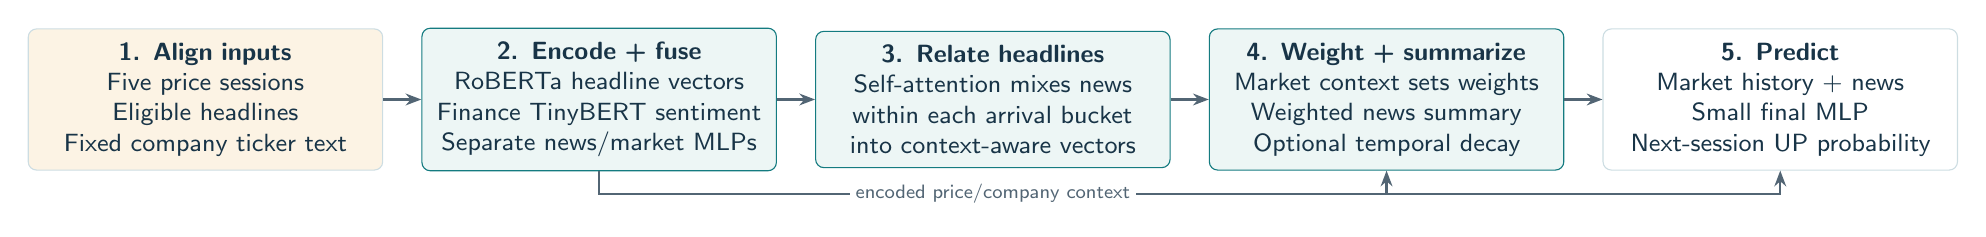
\begin{tikzpicture}[x=1cm,y=1cm]
\node[box,fill=sand] (p1) at (0,0) {\textbf{1. Align inputs}\\Five price sessions\\Eligible headlines\\Fixed company ticker text};
\node[core] (p2) at (5,0) {\textbf{2. Encode + fuse}\\RoBERTa headline vectors\\Finance TinyBERT sentiment\\Separate news/market MLPs};
\node[core] (p3) at (10,0) {\textbf{3. Relate headlines}\\Self-attention mixes news\\within each arrival bucket\\into context-aware vectors};
\node[core] (p4) at (15,0) {\textbf{4. Weight + summarize}\\Market context sets weights\\Weighted news summary\\Optional temporal decay};
\node[box] (p5) at (20,0) {\textbf{5. Predict}\\Market history + news\\Small final MLP\\Next-session UP probability};
\foreach \a/\b in {p1/p2,p2/p3,p3/p4,p4/p5}{\draw[arr](\a)--(\b);}
\draw[arr] (p2.south)--(5,-1.2)--(15,-1.2)--(p4.south);
\draw[arr] (15,-1.2)--(20,-1.2)--(p5.south);
\node[font=\scriptsize,text=slate,fill=white,inner sep=2pt] at (10,-1.2) {encoded price/company context};
\end{tikzpicture}
\end{center}
{\small\textbf{Frozen:} RoBERTa and sentiment models. \textbf{Learned:} text projection, price/sentiment encoders, fusion layers, attention and final MLP. Prices supply the market query and also enter the predictor directly.}

\sub{2a / What actually enters the final MLP?}
\begin{tabularx}{\linewidth}{@{}P{3.55cm}YP{4.5cm}@{}}
\toprule
\textbf{Version} & \textbf{Input to the final predictor} & \textbf{Size / history}\\\midrule
FININ paper, Eq. 7 & Encoded index history (prices + market description) + daily weighted news summaries (Reuters headlines + instrument sentiment) & 1--20 input days; width depends on model\\
Our initial baseline & Five market vectors + five daily news summaries & $5\times16+5\times16=\textbf{160}$\\
Our recent temporal tests & Five market vectors + one news vector pooled across the five buckets & $5\times16+16=\textbf{96}$\\\bottomrule
\end{tabularx}
{\small\textbf{Inside these vectors:} market = prices/volume + ticker context; news = headlines + sentiment, mixed and weighted. Raw sentiment, headline weights and ages are \textbf{not separate final-MLP columns}; they shape the news summary upstream.}

\newpage
\heading{Does news reach the prediction? What do interactions do?}
\sub{3 / Direct evidence of news and weight dependence}
Hold the \textbf{trained network and market inputs fixed}; change only the named news input or attention operation. No retraining in these probes. The examples below use the \textbf{160-input baseline}, forecast date \textbf{31 August 2020}, seed 17.

\begin{tabularx}{\linewidth}{@{}p{1.8cm}rYr@{}}
\toprule
\textbf{Company} & \textbf{Original UP probability} & \textbf{Controlled change} & \textbf{New UP probability}\\\midrule
AEP & 47.73\% (DOWN) & Replace headline vectors with their training mean; retain prices, sentiment and masks & 54.49\% (UP)\\
AEP & 47.73\% (DOWN) & Bypass headline self-attention; retain existing trained weights & 55.56\% (UP)\\
AAPL & 53.64\% (UP) & Replace market-query headline weights with uniform weights & 56.69\% (UP)\\\bottomrule
\end{tabularx}

{\small Across four selected networks and \textbf{44 news-containing validation model-cases}, headline replacement changed 44/44 probabilities; uniform query weighting changed 16/44. These are illustrative sensitivity checks, not retrained forecasting comparisons. The original outputs reproduced saved predictions.}
\callout{\textbf{What this establishes:} the model uses news and attention. \textbf{What it does not establish:} meaningful understanding of the news, or better forecasts. Input substitutions can move a prediction in the wrong direction.}

\begin{minipage}[t]{.48\linewidth}
\sub{5 / How headline interactions work}
Each headline starts as a vector containing text and sentiment. Self-attention replaces it with a learned mixture of the headlines in its bucket. Market-query weighting then combines those \textbf{mixtures}. Interactions run separately within each bucket, not directly between individual headlines across days.

\textbf{Inspecting the Apple example on page 1:}\par
\begin{tabularx}{\linewidth}{@{}Yr@{}}
\toprule
\textbf{Title topic (shortened)} & \textbf{Final bucket weight}\\\midrule
Dow Jones earnings; Apple buy point & 16.5\%\\
Expert warns of stock-market selling & 13.6\%\\
Autos and the chip industry & 18.1\%\\
Dow Jones and consumer confidence & 15.9\%\\
SAP/Deutsche Telekom contact-tracing app & 20.2\%\\
Apple earnings and iPhone sales & 15.6\%\\\bottomrule
\end{tabularx}

{\small\color{slate}These six retained titles mix direct Apple events with broad/other-company topics. This is a title-only inspection; article bodies and discarded stories were not assessed. The largest weight is on a \emph{contextual mixture}, so it is not proof that the SAP story itself matters most.}
\end{minipage}\hfill
\begin{minipage}[t]{.48\linewidth}
\sub{New inspection / Does mixing preserve distinctions?}
We inspected the four saved full-model traces. The table measures how similar headlines' vectors are \textbf{before and after self-attention}: a value near 1 means almost the same direction.

\begin{tabularx}{\linewidth}{@{}Yrr@{}}
\toprule
\textbf{Period / seed} & \textbf{Before} & \textbf{After}\\\midrule
2020 / 17 & 0.418 & 0.9998\\
2020 / 42 & 0.530 & 0.9997\\
2021 / 17 & 0.216 & 0.3665\\
2021 / 42 & 0.834 & 1.0000\\\bottomrule
\end{tabularx}

\textbf{Finding:} in three of four inspected networks, mixing makes headline vectors almost identical in direction. This raises a \textbf{blending/bottleneck concern}, but does not prove useful information was erased. Vector lengths can still differ; the fourth model behaves differently.

{\small\color{slate}Median within-bucket pairwise cosine similarity; 34 multi-headline buckets per model, from two saved first-evaluation snapshot dates. The reconstructed attention outputs match saved vectors. This is a diagnostic, not a semantic or causal test.}

\textbf{New comparison (four fits):} remove \emph{only self-attention}; retain market-query weighting and the same inputs/training settings. Full loss: \textbf{0.690388}; no-interaction loss: \textbf{\NoInteractionLoss}. Removal increases pooled loss by \textbf{\InteractionDelta}, conditional 95\% interval \textbf{\InteractionInterval}. \InteractionVerdict
\end{minipage}

\newpage
\heading{News decay: a negligible effect, with unresolved causes}
\begin{minipage}[t]{.48\linewidth}
\sub{4 / Completed temporal tests}
\textbf{Matched inputs:} same eligible news, five price sessions and 96-input pooled MLP. Equal weighting is compared with a fixed \textbf{48-hour half-life}: every extra 48 hours halves a story's multiplier before normalization. This is news-age weighting, not optimizer weight decay.

\textbf{Evaluation:} 2,004 company-days on 167 distinct dates; May--August 2020 and January--April 2021; two seeds. Lower log loss means better probabilities.

\begin{tabularx}{\linewidth}{@{}Yr@{}}
\toprule
\textbf{Model / reference} & \textbf{Log loss}\\\midrule
Training-prevalence probabilities & 0.689820\\
Prices only (matched pooled geometry) & 0.689771\\
Prices + current arrival bucket & 0.689651\\
Prices + current and older news, equal weighting & 0.690210\\
Prices + current and older news, 48-hour decay & 0.689887\\\bottomrule
\end{tabularx}

Decay improves loss by only \textbf{0.000324}. Its conditional 95\% difference interval is \textbf{[$-0.001176$, $+0.000539$]}, crossing zero. The predeclared practical improvement of 0.005 was not reached. Adding older buckets also failed to improve forecasting reliably.

\textbf{Interpretation:} treat the decay change as \textbf{practically negligible and indistinguishable from noise}. Do not interpret tiny curve bumps as a market discovery.
\end{minipage}\hfill
\begin{minipage}[t]{.48\linewidth}
\sub{What does the age curve measure?}
Remove one age bucket at a time, keep prices/model fixed, and predict again. Plot \textbf{loss after removal minus original loss}.

\begin{center}
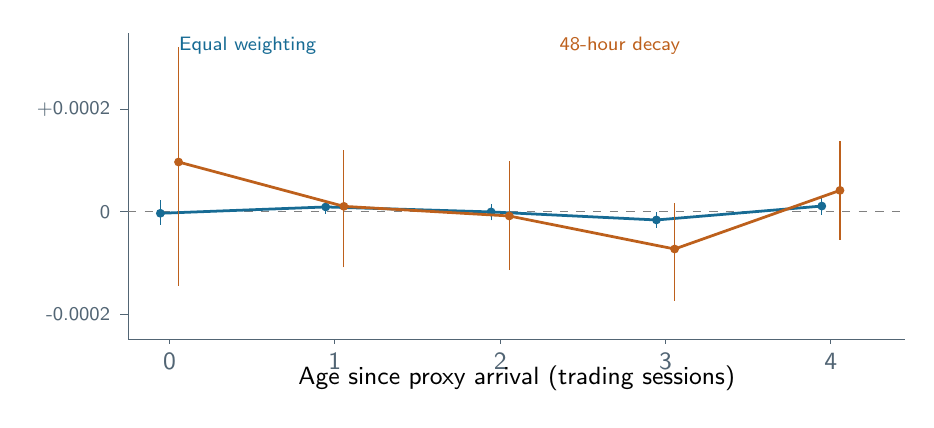
\begin{tikzpicture}[x=2.1cm,y=.65cm]
\draw[slate] (-.25,-2.50000)--(4.45,-2.50000);
\draw[slate] (-.25,-2.50000)--(-.25,3.50000);
\draw[dashed,gray] (-.25,0.00000)--(4.45,0.00000);
\foreach \xx in {0,1,2,3,4}{\draw[slate] (\xx,-2.50000)--(\xx,-2.58000) node[below,font=\small]{\xx};}
\foreach \yy/\lab in {-2/-0.0002,0/0,2/+0.0002}{\draw[slate] (-.25,\yy)--(-.30,\yy) node[left,font=\scriptsize]{\lab};}
\draw[plotblue,line width=1pt] plot coordinates {(-0.055,-0.02812) (0.945,0.09567) (1.945,-0.00154) (2.945,-0.15867) (3.945,0.11294)};
\draw[plotblue] (-0.055,-0.25593)--(-0.055,0.22486);
\fill[plotblue] (-0.055,-0.02812) circle[radius=1.6pt];
\draw[plotblue] (0.945,-0.03425)--(0.945,0.23497);
\fill[plotblue] (0.945,0.09567) circle[radius=1.6pt];
\draw[plotblue] (1.945,-0.16652)--(1.945,0.15033);
\fill[plotblue] (1.945,-0.00154) circle[radius=1.6pt];
\draw[plotblue] (2.945,-0.31363)--(2.945,-0.00722);
\fill[plotblue] (2.945,-0.15867) circle[radius=1.6pt];
\draw[plotblue] (3.945,-0.05471)--(3.945,0.28389);
\fill[plotblue] (3.945,0.11294) circle[radius=1.6pt];
\draw[plotorange,line width=1pt] plot coordinates {(0.055,0.97362) (1.055,0.10721) (2.055,-0.08068) (3.055,-0.72619) (4.055,0.41907)};
\draw[plotorange] (0.055,-1.44330)--(0.055,3.22492);
\fill[plotorange] (0.055,0.97362) circle[radius=1.6pt];
\draw[plotorange] (1.055,-1.08485)--(1.055,1.21059);
\fill[plotorange] (1.055,0.10721) circle[radius=1.6pt];
\draw[plotorange] (2.055,-1.13022)--(2.055,0.98675);
\fill[plotorange] (2.055,-0.08068) circle[radius=1.6pt];
\draw[plotorange] (3.055,-1.73686)--(3.055,0.16944);
\fill[plotorange] (3.055,-0.72619) circle[radius=1.6pt];
\draw[plotorange] (4.055,-0.54751)--(4.055,1.38469);
\fill[plotorange] (4.055,0.41907) circle[radius=1.6pt];
\node[font=\scriptsize,text=plotblue,anchor=west] at (0,3.25000) {Equal weighting};
\node[font=\scriptsize,text=plotorange,anchor=west] at (2.3,3.25000) {48-hour decay};
\node[font=\small] at (2.1,-3.25000) {Age since proxy arrival (trading sessions)};
\end{tikzpicture}
\end{center}

\textbf{Above zero:} removal worsens loss. \textbf{Below zero:} removal improves loss. Age 0 is the current \emph{arrival} bucket, not necessarily freshly published news. Bars are conditional 95\% intervals.

\textbf{Result:} tiny, non-monotonic effects; \textbf{9 of 10 intervals include zero}. Removing news also renormalizes remaining weights. The curve does not estimate an economic news half-life.

{\small\color{slate}Normalized decay tests relative recency: a common age offset cancels. FININ itself has no explicit exponential-decay term; this is an independent extension.}
\end{minipage}

\sub{Why might useful forecasting information be missing?}
\begin{tabularx}{\linewidth}{@{}P{3.5cm}YY@{}}
\toprule
\textbf{Candidate} & \textbf{What we observed} & \textbf{What is still unproven}\\\midrule
Timing / relevance & Date-based D+2 eligibility; mixed headline topics; six-story hash cap & Whether useful information is already priced in or useful stories are excluded\\
Aggregation / learning & Near-identical mixed vectors in three traces. One full fit: training loss $0.6915\to0.6730$, validation $0.6961\to0.6998$ & Whether mixing loses predictive content, or the model fits weak/noisy signals\\\bottomrule
\end{tabularx}
\caution{\textbf{Root cause: not identified.} The news branch is connected; useful generalization remains unproven. A weak effect is not proof of a bug or an unusable dataset. Removing interactions did not rescue performance overall; high vector similarity alone does not justify removing attention.}
\textbf{Next focused step:} audit retained versus discarded headline relevance and timing; test any proposed change under a fixed chronological protocol. Possible final-input additions are explicit relevance, novelty and coverage summaries, but their benefit remains untested.

\vfill
{\scriptsize\color{slate}\textbf{Scope:} these development periods were already inspected; subsequent diagnostics/comparisons are exploratory. Paired intervals retain companies together in five-date blocks and omit training uncertainty. Reserved late-2021 outcomes remain unopened. \textbf{Sources:} saved CMIN baseline, news-dependency, decay, older-news and new interaction studies; \href{https://aclanthology.org/2024.findings-emnlp.189.pdf}{Wang, Cohen \& Ma (2024), FININ, Eqs. 1--7}; \href{https://github.com/BigRoddy/CMIN-Dataset/tree/3f571a53b81d8f3ea7b3afb9877bdbdbeae54c97/CMIN-US}{pinned CMIN-US release}.}
\end{document}
